\documentclass[xcolor={dvipsnames}]{beamer}
\usepackage[utf8]{inputenc}
\usetheme{Rochester}
\beamertemplatenavigationsymbolsempty
\setbeamercolor*{structure}{bg=Mahogany!20,fg=Mahogany}

\setbeamercolor*{palette primary}{use=structure,fg=white,bg=structure.fg}
\setbeamercolor*{palette secondary}{use=structure,fg=white,bg=structure.fg!75}
\setbeamercolor*{palette tertiary}{use=structure,fg=white,bg=structure.fg!50!black}
\setbeamercolor*{palette quaternary}{fg=white,bg=black}

\setbeamercolor{section in toc}{fg=black,bg=white}
\setbeamercolor{alerted text}{use=structure,fg=structure.fg!50!black!80!black}

\setbeamercolor{titlelike}{parent=palette primary,fg=structure.fg!50!black}
\setbeamercolor{frametitle}{bg=Mahogany,fg=white}

\setbeamercolor*{titlelike}{parent=section in toc}
\linespread{0.8}
% \usecolortheme{beaver}

%% Paquetes adicionales
\usepackage{multicol}
\usepackage{ragged2e}
\usepackage{tikz}
\usepackage{minted}
\usepackage{setspace}

\title[Docker: the nice and the gory] {Docker: the nice and the gory}
\author[Leandro Kollenberger]
{Leandro Kollenberger}
\institute[redbee] {
redbee studios
}
\date[dockerpres] {
	6 de Abril de 2018
}
\subject {Docker: the gory details}
\titlegraphic{\vspace{-2cm}}
% \titlegraphic{
\includegraphics[height=.5\textheight]{assets/docker_logo.png}}

\pgfdeclareimage[height=0.5cm]{left-logo}{assets/redbee_logo.png}

\setbeamertemplate{sidebar left}
{
\logo{\pgfuseimage{left-logo}}
\vfill%
\rlap{\hskip0.1cm\insertlogo}%
%\vskip15pt%
\vskip5pt%
}

\begin{document}

\begin{frame}
	 \tikz [remember picture,overlay]
		\node at
				% ([yshift=3cm]current page.south) 
				([yshift=1.8cm]current page.center)
				{
\includegraphics[height=.5\textheight]{assets/docker_logo.png}};
	 \titlepage
\end{frame}

% \frame{\titlepage}

\begin{frame}[fragile]
	\frametitle{Por qué presenciar esta charla}
	\begin{itemize}
		\item Sos desarrollador, usás Docker hace tiempo en tu día a día pero te interesa saber algo más de detalle.
		\item Sos de ops, pero nunca tocaste Docker a fondo.
		\item Te interesó la charla.
		\item Hay comida.
	\end{itemize}
\end{frame}

\begin{frame}[fragile]
	\frametitle{¿Qué es Docker?}
	\vspace{-0.8cm}
	\begin{multicols}{2}
	\justify
		Docker es una herramienta que nos facilita enpaquetar una aplicación junto con su \textit{runtime} dentro de una \textbf{imagen}, que luego se ejecutará dentro de un \textbf{container}.

		Gracias a la gran cantidad de \textbf{imágenes base} que hay disponibles en el \textbf{Docker Hub} y la simple sintaxis del \textbf{Dockerfile}, crear imágenes propias con nuestra aplicación es muy simple.
	\columnbreak
	\vspace*{\fill}
		\textbf{Dockerfile}
		\begin{minted}{docker}
FROM debian:9
RUN echo "echo 'Hola mundo!'"\
		> /hi.sh && \
		chmod +x /hi.sh
ENTRYPOINT hi.sh
		\end{minted}
	\vspace*{\fill}
	\end{multicols}
\end{frame}

\begin{frame}[fragile]
	\Huge The nice about Docker
\end{frame}

\begin{frame}[fragile]
	\frametitle{Usando la CLI}
	Comandos útiles para manejar Docker
	\begin{itemize}
		\item \texttt{docker run}: crear un container. Optiones útiles:
		\begin{itemize}
			\item \texttt{--rm}: borrar el container cuando se detenga.
			\item \texttt{-i}: \textit{interactive}, habilita la salida estándar del container.
			\item \texttt{-t}: habilita la entrada de teclado al container, generalmente usado junto con \texttt{-i}.
			\item \texttt{-p puertoexterno:puertointerno}: \textit{publish}, publica (mapea) un puerto externo en el host a un puerto dentro del container, por ejemplo \texttt{-p 8080:80} mapea las conexiones entrantes en el puerto 8080 del host al 80 del container.
			\item \texttt{--name=lalala} \textit{self-explainatory}.
			\item \texttt{-v /path/en/el/host:/path/dentro/del/container} \textit{volume}, mapea un volúmen de docker o path en el host a un path dentro del container. Sirve también para archivos y se le puede agregar \texttt{:ro} para indicar \textit{read-only}.
		\end{itemize}
	\end{itemize}
\end{frame}

\begin{frame}[fragile]
	\frametitle{Usando la CLI}
	\begin{itemize}
		\item \texttt{docker ps}: Listar containers corriendo (con \texttt{-a} lista también containers detenidos)
		\item \texttt{docker start/stop}: Arrancar/detener containers.
		\item \texttt{docker images}: Listar imágenes disponibles en el sistema.
		\item \texttt{docker rmi}: Borrar imágenes.
		\item \texttt{docker network}: Listar/borrar/crear una network administrada por Docker.
		\item \texttt{docker exec -it container comando}: Ejecutar \texttt{comando} dentro de \texttt{container}. Sirve para "meterse" dentro y hacer cambios.
	\end{itemize}
\end{frame}

\begin{frame}[fragile]
	\frametitle{Docker Compose}
	 \vspace{-0.4cm}
	\begin{multicols}{2}
	% \justify
	\vspace*{\fill}
	Hermoso.

	Es un archivo YAML que describe containers a crear. Permite comunicación entre containers con nombre de DNS y sin linkear.

	\scriptsize Sintaxis: https://docs.docker.com/compose/compose-file/
	\vspace*{\fill}
	\columnbreak
	% \vspace{2}
	\tiny \begin{minted}{yaml}
version: "2"
services:
  nginx:
    image: nginx:latest
    restart: unless-stopped
    ports:
      - "80:80"
      - "443:443"
    networks:
      - web
    volumes:
      - /data/ssl:/ssl:ro
      - /data/nginx.conf:/data/nginx.conf:ro
  nextcloud:
    image: nextcloud:apache
    restart: unless-stopped
    volumes:
      - /data/nextcloud:/var/www/html/data
    expose:
      - "80"
    networks:
      - web
    depends_on:
      - nginx
      - nextcloud-db
  nextcloud-db:
    image: postgres:latest
    restart: unless-stopped
    environment:
      - "POSTGRES_PASSWORD=******"
      - "POSTGRES_USER=nextcloud"
      - "POSTGRES_DB=nextcloud"
    volumes:
      - /data/nextcloud-db:/var/lib/postgresql/data
    expose:
      - "5432"
    networks:
      - web
		\end{minted}
	\vspace*{\fill}
	\end{multicols}
\end{frame}

\begin{frame}[fragile]
	\Huge The \textbf{gory} about Docker
\end{frame}

\begin{frame}[fragile]
	\frametitle{¿Qué es un container?}
	\vspace{-0.8cm}
	\begin{multicols}{2}
	\justify
			\begin{spacing}{0.8}
		\small Un \textbf{container} es una funcionalidad del sistema operativo que nos permite ejecutar ciertas aplicaciones dentro de un \textbf{namespace} aparte.

		\vspace{0.25cm}

		\small Un \textbf{namespace} es una separación lógica de los recursos del sistema, como por ejemplo CPU, memoria RAM, puntos de montaje (disco), árbol de procesos, network, etc.

		\vspace{0.25cm}

		\small De esta forma un container nos provee seguridad y aislamiento de las aplicaciones que corren en él, similar a lo que nos permite una VM, sin el overhead de simular hardware y correr un sistema operativo entero, ya que todos los containers corriendo en un mismo host comparten su kernel.
			\end{spacing}
	\columnbreak
	\vspace*{\fill}
		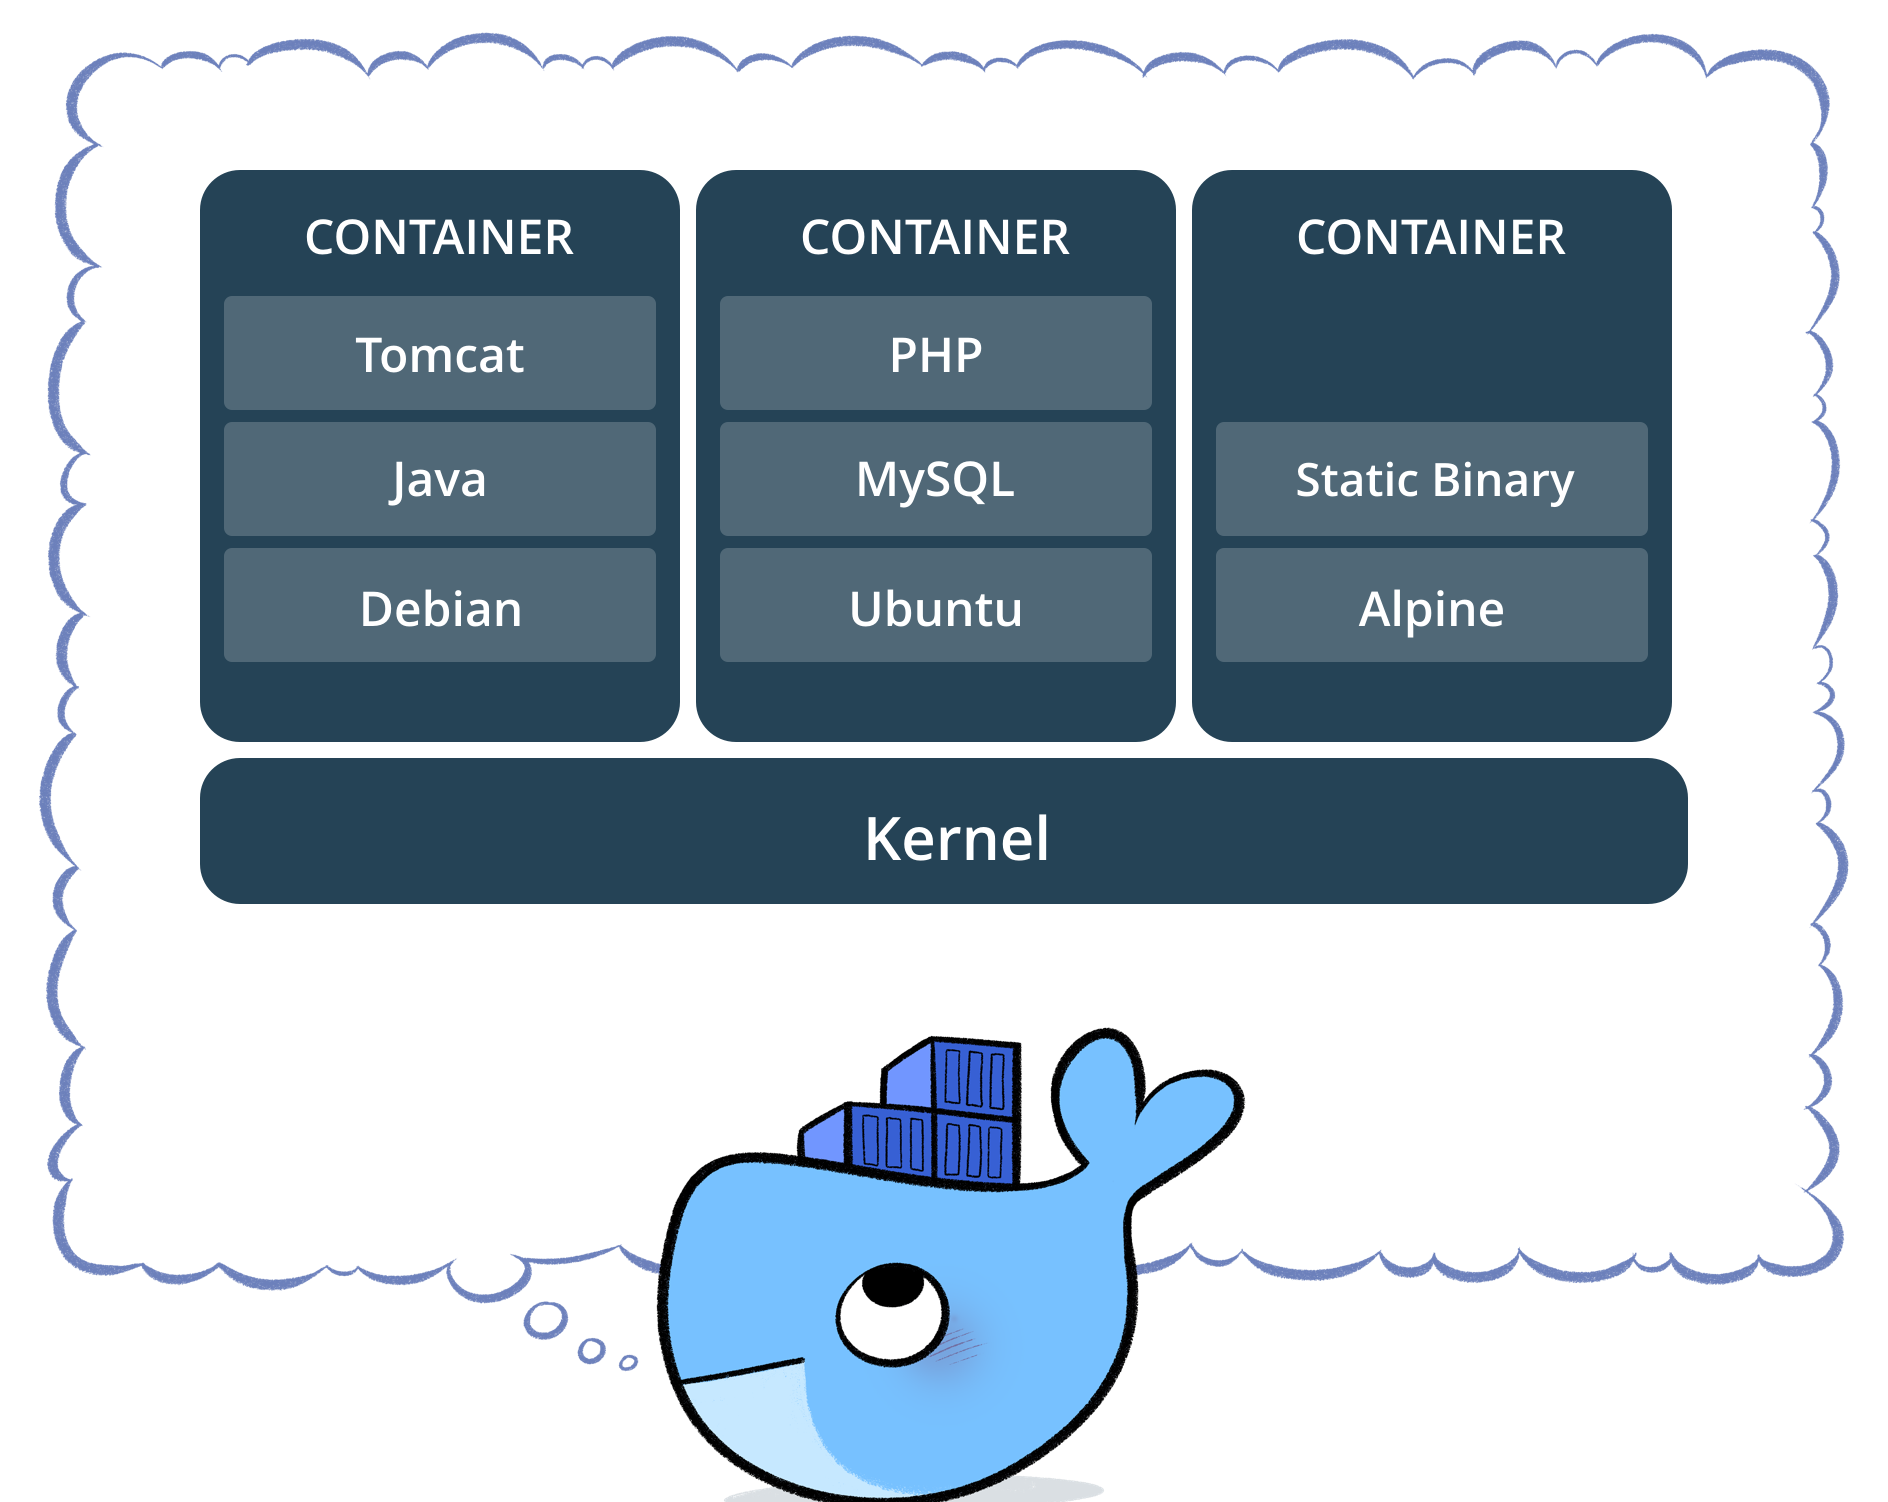
\includegraphics[height=.6\textheight]{assets/containerz.png}
	\vspace*{\fill}
	\end{multicols}
\end{frame}

\begin{frame}[fragile]
	\frametitle{El concepto de "layer"}
	\vspace{-0.5cm}
	\justify
	\centering
	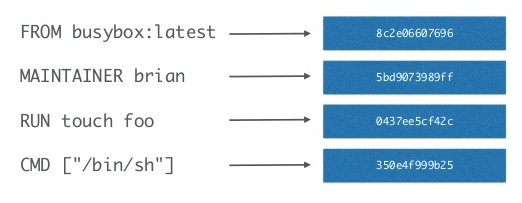
\includegraphics[width=.75\textwidth]{assets/layers3.png}
	\vspace{-0.5cm}
	\begin{multicols}{2}
	\justify
		\begin{spacing}{0.8}
		\small Las imágenes de Docker que podemos usar a diario están compuestas por una o más \textbf{layers}. Éstas imágenes contienen un sistema de archivos correspondiente al sistema operativo o la aplicación que queremos ejecutar. Esta imagen está identificada por un hash y opcionalmente uno o más \textbf{tags}, como por ejemplo \textit{redis:4.0.6} o \textit{debian:latest}.

		\columnbreak

		\small Cada layer contiene únicamente los cambios (ya sean archivos, comandos o metadatos) con respecto a la layer anterior, se identifican con un hash y corresponden cada una a un comando del Dockerfile. Todas las layers que componen una imagen son \textbf{read only}.

		\end{spacing}
	\end{multicols}
\end{frame}

\begin{frame}[fragile]
	\frametitle{El concepto de "layer"}
	\vspace{-0.8cm}
	\begin{multicols}{2}
	\justify
	\vspace*{\fill}
		\hspace{-0.5cm}
		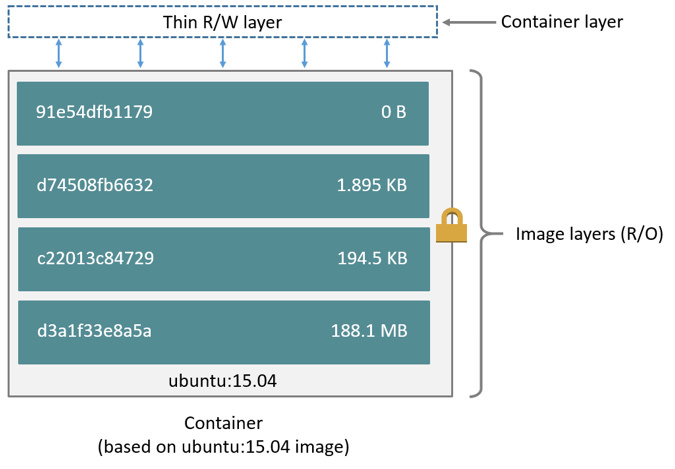
\includegraphics[height=.5\textheight]{assets/layers2.jpg}
	\vspace*{\fill}
	\columnbreak
	\vspace*{\fill}
		\begin{spacing}{0.8}
		\small Cada layer contiene únicamente los cambios (ya sean archivos, comandos o metadatos) con respecto a la layer anterior, se identifican con un hash y corresponden cada una a un comando del Dockerfile. Todas las layers que componen una imagen son \textbf{read only}.

		\vspace{0.25cm}

		\small Al momento de crear un nuevo container a base de una imagen, se crea una pequeña layer \textbf{read-write}, que contiene los cambios creados por el container en ejecución (por ejemplo, por la aplicación).

		\vspace{0.25cm}

		\small Esta última layer se \textbf{pierde al eliminar el container}.
			\end{spacing}
	\vspace*{\fill}
	\end{multicols}
\end{frame}

\begin{frame}[fragile]
	\frametitle{Arquitectura de Docker}
	\centering
		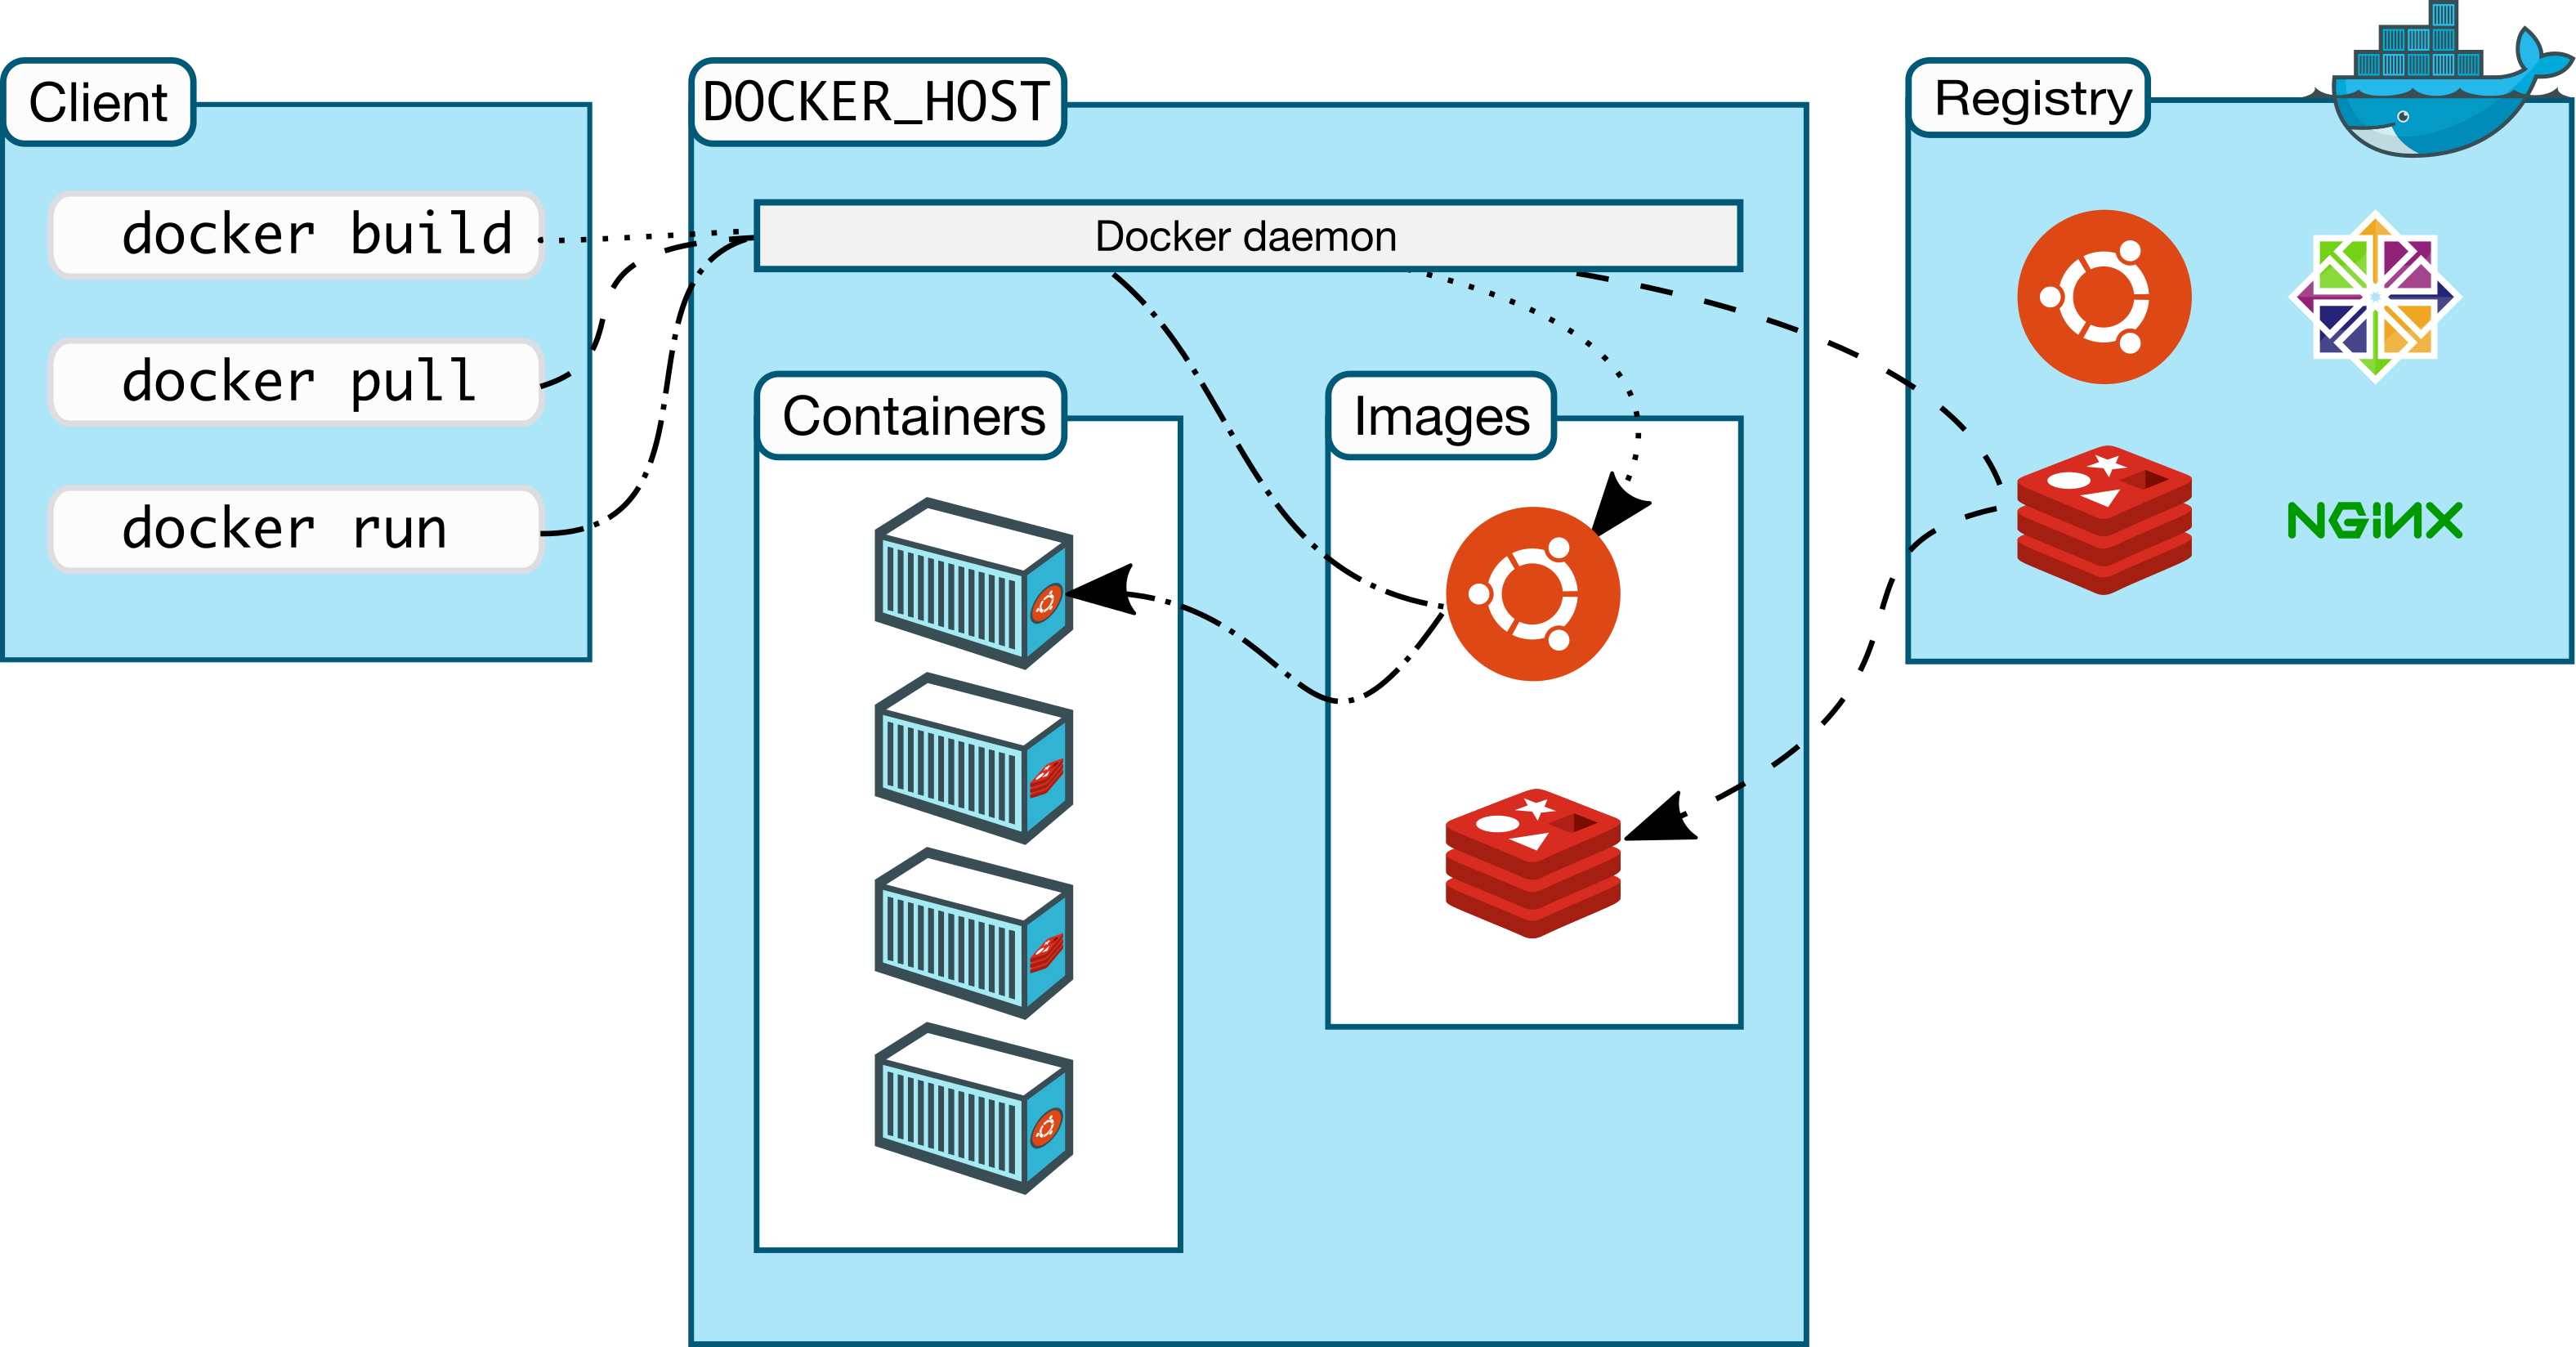
\includegraphics[width=\textwidth]{assets/architecture.png}
\end{frame}

\begin{frame}[fragile]
	\frametitle{Arquitectura de Docker}
	\begin{itemize}
		\item \footnotesize Cliente: Aplicación de consola que se comunica con el daemon. Puede comunicarse tanto con el daemon de la máquina local (por socket de Unix) como con una remota (por TCP). Ejemplo: \texttt{docker run}, \texttt{docker image ls}.
		\item \footnotesize Daemon: Servicio de Docker corriendo en backgroud que gestiona imágenes y containers.
		\item \footnotesize Registry: Repositorio remoto de imágenes. En detalle, almacena tres tipos de datos:
		\begin{itemize}
			\item \footnotesize Layers (cada una con su hash y el comando de Dockerfile que la generó).
			\item \footnotesize Imágenes, básicamente una lista de hashes de cada una de las layers que la componen, más metadatos y un hash propio de la imagen.
			\item \footnotesize Tags (human readable), que apuntan a hashes de imágenes. Son sobreescribibles. Ejemplos: \texttt{redis:4.0.6}, \texttt{jess/routersploit} o \texttt{docker.dev.redbee.io/ms-lalala-rest:release-v1.2.1}. Pueden referirse a la library (imágenes oficiales, primer caso), imágenes dentro del Docker Hub pero de terceros (segundo caso) u otras registries privadas (tercer caso). Si no se indica una versión por defecto es \texttt{latest}.
		\end{itemize}
	\end{itemize}
\end{frame}

\begin{frame}[fragile]
	\frametitle{Namespaces}
	El \textit{kernel} Linux nos permite aislar los siguientes subsistemas en namespaces:
	\begin{itemize}
		\item \textbf{mnt}, Mount: puntos de montaje y sistema de archivos.
		\item \textbf{pid}, Process ID: árbol de procesos.
		\item \textbf{net}, Network: placas de red, tablas de routeo, firewall...
		\item \textbf{ipc}, Inter-process Communication: colas, pilas, sockets...
		\item \textbf{uts}: hostname, domain name.
		\item \textbf{user}: IDs de usuario y grupo.
	\end{itemize}
	% Nos vamos a enfocar en \textbf{mnt}, \textbf{pid}, \textbf{net} y \textbf{user}.
\end{frame}

\begin{frame}[fragile]
	\frametitle{Networking en containers}
	Las aplicaciones en general publican servicios, cómo accedemos si estamos dentro de un container?
	\begin{itemize}
		\item \texttt{net=host}: desactivamos el namespace de networking, comparte puertos y servicios con las aplicaciones comúnes del host.
		\item \texttt{net=bridge}: ponemos un switch virtual en el host, placas de red dentro del container, las conectamos ahí y abrimos puertos en el host. Funciona parecido a un router hogareño: comparte una IP (la del host) y forwardea puertos a donde corresponda. Ejemplo: \texttt{docker run -d -p 1234:80 nginx} levanta un container de nginx y forwardea conexiones entrantes al host en puerto 1234 al puerto 80 del container.
		\item \texttt{net=none}: desactiva la red completamente, \textit{duh.}
	\end{itemize}
\end{frame}

\begin{frame}[fragile]
	\frametitle{Storage drivers (\textit{a.k.a. La magia detrás de las layers})}
	Los storage drivers (también conocidos como \textit{graph drivers}) son drivers del kernel Linux que permiten montar las layers una encima de otra, agregando cada una sus respectivos cambios. Opciones:
	\begin{itemize}
		\item \texttt{overlay2}: Recomendada, es la más moderna.
		\item \texttt{overlay}: Recomendada (si el kernel no soporta \texttt{overlay2}).
		\item \texttt{aufs}: Vieja, se usaba antes de que existiera \texttt{overlay}). No recomendada.
		\item \texttt{btrfs}
		\item \texttt{devicemapper}:
		\begin{itemize}
			\item \texttt{direct-lvm}: Recomendada en caso de tener LVM con thinpool.
			\item \texttt{direct-loop}: No recomendada, lentísima.
		\end{itemize}
	\end{itemize}
\end{frame}

\begin{frame}[fragile]
	\frametitle{Más allá de Docker}
	Los containers son divertidos, pero complejos de administrar!
	\begin{itemize}
		\item Kubernetes.
		\item Apache Mesos.
		\item Hashicorp Nomad.
		\item Docker Swarm.
	\end{itemize}
\end{frame}

%% Fin de la presentación!
\begin{frame}
	\vspace{-0.8cm}
	\begin{center}
		%% Foto de Perón
		\begin{figure}
		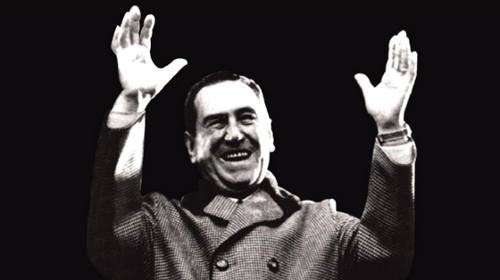
\includegraphics[width = 0.8\textwidth]{./assets/peron1.jpg}
		\end{figure}
		\Large{\textbf{Gracias! \\ Preguntas?}}
	\end{center}
\end{frame}

\end{document}
